\documentclass[conference]{IEEEtran}
\usepackage{cite}
\usepackage{amsmath,amssymb,amsfonts}
\usepackage{algorithmic}
\usepackage{graphicx}
\usepackage{textcomp}
\usepackage{xcolor}
\usepackage{booktabs}
\usepackage{multirow}
\usepackage{hyperref}
\hypersetup{
    colorlinks=true,
    linkcolor=blue,
    filecolor=magenta,      
    urlcolor=cyan,
    pdftitle={ResGIN for PPI Prediction},
    pdfpagemode=FullScreen,
    }

\begin{document}

\title{Enhancing Protein-Protein Interaction Prediction with Residual Graph Isomorphism Networks}

\author{\IEEEauthorblockN{Author Name}
\IEEEauthorblockA{Department of Computer Science\\
Institution Name\\
City, Country\\
email@example.com}}

\maketitle

\begin{abstract}
Protein-protein interaction (PPI) prediction remains a challenging problem in computational biology. While graph neural networks (GNNs) have shown promising results in this domain, there is still room for architectural improvements to better capture the complex relationships between protein structures. In this paper, we introduce a novel architecture called Residual Graph Isomorphism Network (ResGIN) for PPI prediction. ResGIN combines the expressive power of Graph Isomorphism Networks with residual connections to enable deeper networks and improved gradient flow during training. We compare ResGIN against state-of-the-art GNN architectures, namely Graph Convolutional Neural Networks (GCNN) and Graph Attention Networks (GAT). Our comprehensive experiments demonstrate that ResGIN achieves competitive performance and exhibits strong learning capacity even with limited training epochs. This work contributes a new architectural approach for modeling protein structures as graphs and predicting their interactions with high accuracy.
\end{abstract}

\begin{IEEEkeywords}
protein-protein interaction, graph neural networks, graph isomorphism networks, residual connections, deep learning
\end{IEEEkeywords}

\section{Introduction}
Protein-protein interactions (PPIs) play a fundamental role in numerous biological processes and are essential for understanding cellular function, disease mechanisms, and drug discovery. Experimental methods for determining PPIs are often time-consuming, expensive, and may yield high false-positive rates \cite{skrabanek2008computational}. Thus, computational approaches for predicting PPIs have gained significant attention in recent years.

Graph neural networks (GNNs) have emerged as powerful tools for modeling relationships in non-Euclidean data structures such as protein graphs \cite{gainza2020deciphering}. By representing proteins as graphs—where nodes correspond to amino acids and edges represent their spatial or sequential relationships—GNNs can learn meaningful representations that capture both local and global structural information relevant to interaction prediction.

Previous approaches have utilized various GNN architectures for PPI prediction, with Graph Convolutional Neural Networks (GCNNs) \cite{kipf2017semi} and Graph Attention Networks (GATs) \cite{velivckovic2018graph} being among the most prominent. While these approaches have demonstrated significant success, they face challenges in modeling very deep networks due to issues such as vanishing gradients.

In this paper, we introduce a novel architecture called Residual Graph Isomorphism Network (ResGIN) for PPI prediction. ResGIN combines the theoretical power of Graph Isomorphism Networks (GINs) \cite{xu2018powerful} with residual connections \cite{he2016deep} to enable deeper networks and improved gradient flow during training. The GIN architecture has been shown to be as powerful as the Weisfeiler-Lehman graph isomorphism test in distinguishing graph structures, making it particularly suitable for capturing the complex structural patterns in proteins.

We conduct comprehensive experiments comparing ResGIN against GCNN and GAT models on a human protein-protein interaction dataset. Our results demonstrate that ResGIN achieves competitive performance, even with limited training, suggesting its potential for further improvements with extended optimization.

\section{Related Work}
\subsection{Graph Neural Networks for PPI Prediction}
Graph-based approaches for protein analysis have gained popularity due to their ability to capture structural information in a natural way. Several studies have applied various GNN architectures to PPI prediction. For instance, \cite{fout2017protein} proposed a graph convolutional network for predicting protein interfaces by extracting features from local neighborhoods in protein graphs. \cite{gligorijevic2019structure} introduced DeepFRI, which combines GCNs with sequence information to predict protein functions.

\subsection{Residual Networks}
Residual networks \cite{he2016deep} were introduced to address the degradation problem in very deep neural networks by incorporating skip connections that allow gradients to flow more efficiently during backpropagation. This concept has been adapted to various neural network architectures, including GNNs. For instance, \cite{li2019deepgcns} proposed DeepGCNs, which incorporate residual connections into graph convolutional networks to enable deeper architectures.

\subsection{Graph Isomorphism Networks}
Graph Isomorphism Networks (GINs) \cite{xu2018powerful} were designed to maximize the representational power of GNNs. The authors demonstrated that GINs can distinguish different graph structures at least as well as the Weisfeiler-Lehman isomorphism test, making them theoretically more powerful than many other GNN variants. This property is particularly valuable in the context of protein structure analysis, where capturing subtle structural differences can be crucial for predicting interactions.

\section{Materials and Methods}
\subsection{Dataset}
We utilize a human protein-protein interaction dataset consisting of protein pairs labeled as interacting or non-interacting. Each protein is represented as a graph, where nodes correspond to amino acids with features derived from protein sequence embeddings using SeqVec \cite{heinzinger2019modeling}. Node features are 1024-dimensional vectors capturing contextualized information about each amino acid in the protein sequence. Edges represent spatial proximity between amino acids, with a threshold of 10 Å used to establish connections.

\subsection{Model Architecture}
\subsubsection{Residual Graph Isomorphism Network (ResGIN)}
The proposed ResGIN model combines the expressive power of Graph Isomorphism Networks with residual connections to enable deeper and more effective learning. 

In our approach, proteins are represented as graphs $G = (V, E)$, where $V$ is the set of nodes representing amino acids and $E$ is the set of edges representing spatial relationships between amino acids. Each node $v \in V$ has a feature vector $\mathbf{h}_v \in \mathbb{R}^{1024}$ derived from SeqVec embeddings, capturing the contextual properties of that amino acid within the protein structure.

The ResGIN architecture consists of four primary components:

\begin{itemize}
    \item \textbf{Embedding layers}: Dense linear transformations that project the initial 1024-dimensional node features into a lower-dimensional latent space $\mathbb{R}^{128}$.
    
    \item \textbf{Graph Isomorphism Network (GIN) layers with residual connections}: A sequence of message-passing layers that update node representations based on both their own features and those of their neighbors.
    
    \item \textbf{Global pooling}: A mechanism to aggregate node-level features into a single graph-level representation.
    
    \item \textbf{Interaction prediction module}: Fully connected layers that process the concatenated representations of two proteins to predict their interaction probability.
\end{itemize}

\paragraph{GIN Layer Formulation}
The core component of our architecture is the Graph Isomorphism Network layer. For each node $i$, the GIN layer updates its representation according to:

\begin{equation}
\mathbf{h}_i^{(l+1)} = \text{MLP}^{(l)}\left((1 + \epsilon^{(l)}) \cdot \mathbf{h}_i^{(l)} + \sum_{j \in \mathcal{N}(i)} \mathbf{h}_j^{(l)}\right)
\end{equation}

where $\mathbf{h}_i^{(l)}$ represents the feature vector of node $i$ at layer $l$, $\mathcal{N}(i)$ denotes the neighbors of node $i$, $\epsilon^{(l)}$ is a learnable scalar parameter that adjusts the importance of the central node's features relative to its neighbors, and $\text{MLP}^{(l)}$ is a multi-layer perceptron.

The GIN layer is theoretically more expressive than conventional graph convolutional networks because it can distinguish different graph structures at least as well as the Weisfeiler-Lehman graph isomorphism test. This property is particularly valuable for protein structure analysis, where capturing subtle structural differences is crucial for predicting interactions.

\paragraph{Residual Connection Integration}
In the ResGIN architecture, we enhance the standard GIN layers with residual connections. After each GIN operation, the input features are added to the output:

\begin{equation}
\mathbf{h}_i^{(l+1)} = \mathbf{h}_i^{(l)} + \text{GINConv}(\mathbf{h}_i^{(l)}, \mathcal{N}(i))
\end{equation}

This residual connection is followed by a non-linear activation function and regularization:

\begin{equation}
\mathbf{h}_i^{(l+1)} = \text{ReLU}(\mathbf{h}_i^{(l+1)})
\end{equation}

\begin{equation}
\mathbf{h}_i^{(l+1)} = \text{Dropout}(\mathbf{h}_i^{(l+1)})
\end{equation}

These residual connections offer several important advantages:
\begin{itemize}
    \item They facilitate gradient flow during backpropagation, mitigating the vanishing gradient problem that often affects deep neural networks.
    \item They allow the model to learn incremental transformations of the node features, rather than having to learn complete feature mappings from scratch in each layer.
    \item They enable the construction of deeper networks with stable training characteristics, which is particularly important for capturing complex structural patterns in proteins.
\end{itemize}

\paragraph{Global Pooling and Interaction Prediction}
After processing the protein graphs through multiple GIN layers with residual connections, we apply global mean pooling to obtain fixed-size graph-level representations:

\begin{equation}
\mathbf{h}_G = \frac{1}{|V|} \sum_{v \in V} \mathbf{h}_v^{(L)}
\end{equation}

where $\mathbf{h}_G$ is the graph-level representation and $\mathbf{h}_v^{(L)}$ is the final node representation after $L$ layers.

For predicting protein-protein interactions, we concatenate the graph-level representations of the two proteins and pass them through fully connected layers:

\begin{equation}
\mathbf{z} = [\mathbf{h}_{G_1} \parallel \mathbf{h}_{G_2}]
\end{equation}

\begin{equation}
p = \sigma(f_{\theta}(\mathbf{z}))
\end{equation}

where $\mathbf{h}_{G_1}$ and $\mathbf{h}_{G_2}$ are the graph-level representations of the two proteins, $\parallel$ denotes concatenation, $f_{\theta}$ represents the fully connected neural network layers, $\sigma$ is the sigmoid activation function, and $p$ is the predicted probability of interaction between the two proteins.

\subsubsection{Implementation Details}
Our ResGIN implementation incorporates several important architectural and optimization choices:

\paragraph{Network Architecture}
We employ 4 GIN layers with residual connections. The multi-layer perceptron within each GIN layer follows a bottleneck architecture:
\begin{itemize}
    \item An expansion layer that projects the 128-dimensional input to 256 dimensions
    \item A batch normalization layer to stabilize training
    \item A ReLU activation function to introduce non-linearity
    \item A projection layer that returns the representation to 128 dimensions
\end{itemize}

This bottleneck structure allows the network to create more complex feature transformations while maintaining computational efficiency. The learnable parameter $\epsilon$ in each GIN layer is initialized to 0.1 and optimized during training.

\paragraph{Parameter Details}
The ResGIN model contains approximately 280,000 trainable parameters distributed as follows:
\begin{itemize}
    \item \textbf{Embedding layers}: $\sim$262,144 parameters (2 proteins × 1024 × 128 dimensions)
    \item \textbf{GIN layers}: $\sim$16,384 parameters for each protein (4 layers × [128 × 256 + 256 × 128 + batch norm parameters])
    \item \textbf{Prediction layers}: $\sim$21,312 parameters (256 × 64 + 64 × 1 + bias terms)
\end{itemize}

The majority of parameters reside in the embedding layers, which transform the high-dimensional protein features into the model's working latent space. Despite the relative complexity of the architecture, the parameter count remains reasonable, making the model practical for training on standard hardware.

\paragraph{Information Flow}
The processing of protein data through the ResGIN architecture follows a systematic pipeline:
\begin{enumerate}
    \item Each protein graph is independently processed through parallel branches
    \item Within each branch:
    \begin{itemize}
        \item Node features are embedded into a lower-dimensional latent space
        \item Four sequential GIN layers with residual connections extract hierarchical structural information
        \item After each GIN layer, ReLU activation and dropout are applied
        \item Global mean pooling creates a fixed-size representation of the protein
    \end{itemize}
    \item The representations of both proteins are concatenated into a single vector
    \item This concatenated vector passes through three fully connected layers (dimensions: 256 → 64 → 1)
    \item A sigmoid function produces the final interaction probability
\end{enumerate}

This processing flow enables the model to capture both the internal structural properties of each protein and their potential compatibility for interaction.

\paragraph{Optimization Strategy}
For training, we utilize:
\begin{itemize}
    \item Binary cross-entropy loss to measure prediction error
    \item RAdam optimizer (Rectified Adam) with learning rate 0.0005
    \item ReduceLROnPlateau scheduler to adaptively decrease the learning rate when validation performance plateaus
    \item Early stopping with a patience of 3 epochs to prevent overfitting
    \item Dropout with a rate of 0.2 for regularization
\end{itemize}

This optimization strategy balances efficient training with generalization capability.

\paragraph{Theoretical Advantages}
The ResGIN architecture offers several theoretical advantages for protein-protein interaction prediction:

\begin{itemize}
    \item \textbf{Structural expressivity}: GIN layers can distinguish between different protein graph structures more effectively than standard GCN or GAT layers, capturing subtle structural patterns that may be relevant for interactions.
    
    \item \textbf{Efficient gradient flow}: Residual connections enable more effective backpropagation, allowing for deeper networks that can learn more complex feature hierarchies.
    
    \item \textbf{Regularization}: The combination of batch normalization, dropout, and residual connections helps prevent overfitting, which is particularly important given the complex nature of protein structures and the limited availability of labeled data.
    
    \item \textbf{Adaptability}: The architecture scales well to proteins of different sizes due to the global pooling operation, making it suitable for diverse proteomes.
\end{itemize}

\section{Baseline Models}
We compare the proposed ResGIN model against two strong baseline GNN architectures:

\begin{itemize}
    \item \textbf{Graph Convolutional Neural Network (GCNN)}: A model based on the graph convolutional operator proposed by Kipf and Welling \cite{kipf2017semi}, which aggregates information from neighboring nodes through a normalized adjacency matrix.
    
    \item \textbf{Graph Attention Network (AttGNN)}: A model that employs attention mechanisms to weigh the importance of different neighboring nodes dynamically during message passing \cite{velivckovic2018graph}.
\end{itemize}

\subsection{Training Procedure}
All models were trained using binary cross-entropy loss with the following hyperparameters:

\begin{itemize}
    \item Optimizer: RAdam (Rectified Adam) \cite{liu2019variance}
    \item Learning rate: 0.0005
    \item Batch size: 32
    \item Learning rate scheduler: ReduceLROnPlateau
    \item Early stopping patience: 3-10 epochs (varies by experiment)
\end{itemize}

We conducted both short (5 epochs) and extended training experiments to evaluate the learning efficiency and ultimate performance of each model architecture.

\subsection{Evaluation Metrics}
Models were evaluated using multiple performance metrics:

\begin{itemize}
    \item Accuracy: Percentage of correctly classified protein pairs
    \item Area Under the Receiver Operating Characteristic curve (AUROC)
    \item Precision: Ratio of true positives to predicted positives
    \item Recall (Sensitivity): Ratio of true positives to actual positives
    \item Specificity: Ratio of true negatives to actual negatives
    \item F1 Score: Harmonic mean of precision and recall
    \item Matthews Correlation Coefficient (MCC): A balanced measure accounting for all confusion matrix categories
\end{itemize}

\section{Results and Discussion}

\subsection{Performance Comparison}
Table \ref{tab:model_comparison} presents a comprehensive comparison of the three models after training. The GCNN was trained for 5 epochs, ResGIN for 5 epochs, and AttGNN for 23 epochs (with early stopping).

\begin{table}[ht]
\centering
\caption{Performance comparison of GCNN, ResGIN, and AttGNN models}
\label{tab:model_comparison}
\begin{tabular}{lcccc}
\toprule
\textbf{Metric} & \textbf{GCNN} & \textbf{ResGIN} & \textbf{AttGNN} \\
 & \textbf{(5 epochs)} & \textbf{(5 epochs)} & \textbf{(23 epochs)} \\
\midrule
Validation Accuracy (\%) & 97.21 & 94.89 & 98.22 \\
AUROC & 0.9819 & 0.9768 & 0.9822 \\
Precision & 0.9819 & 0.9529 & 0.9872 \\
Recall/Sensitivity & 0.9801 & 0.9789 & 0.9887 \\
Specificity & 0.9500 & 0.8660 & 0.9644 \\
F1 Score & 0.9810 & 0.9657 & 0.9879 \\
MCC & 0.9285 & 0.8669 & 0.9543 \\
\bottomrule
\end{tabular}
\end{table}

The results show that while ResGIN achieves slightly lower performance metrics than GCNN after 5 epochs of training, it still demonstrates impressive predictive capability with 94.89\% accuracy and an F1 score of 0.9657. The AttGNN model, which was trained for significantly longer (23 epochs), achieves the highest overall performance.

\subsection{Learning Efficiency Analysis}
Fig. \ref{fig:learning_curves} shows the learning curves of the ResGIN model during the 5-epoch training period. The rapid convergence of both training and validation curves suggests that ResGIN learns efficiently and could potentially achieve higher performance with additional training epochs.

\begin{figure}[htbp]
\centering
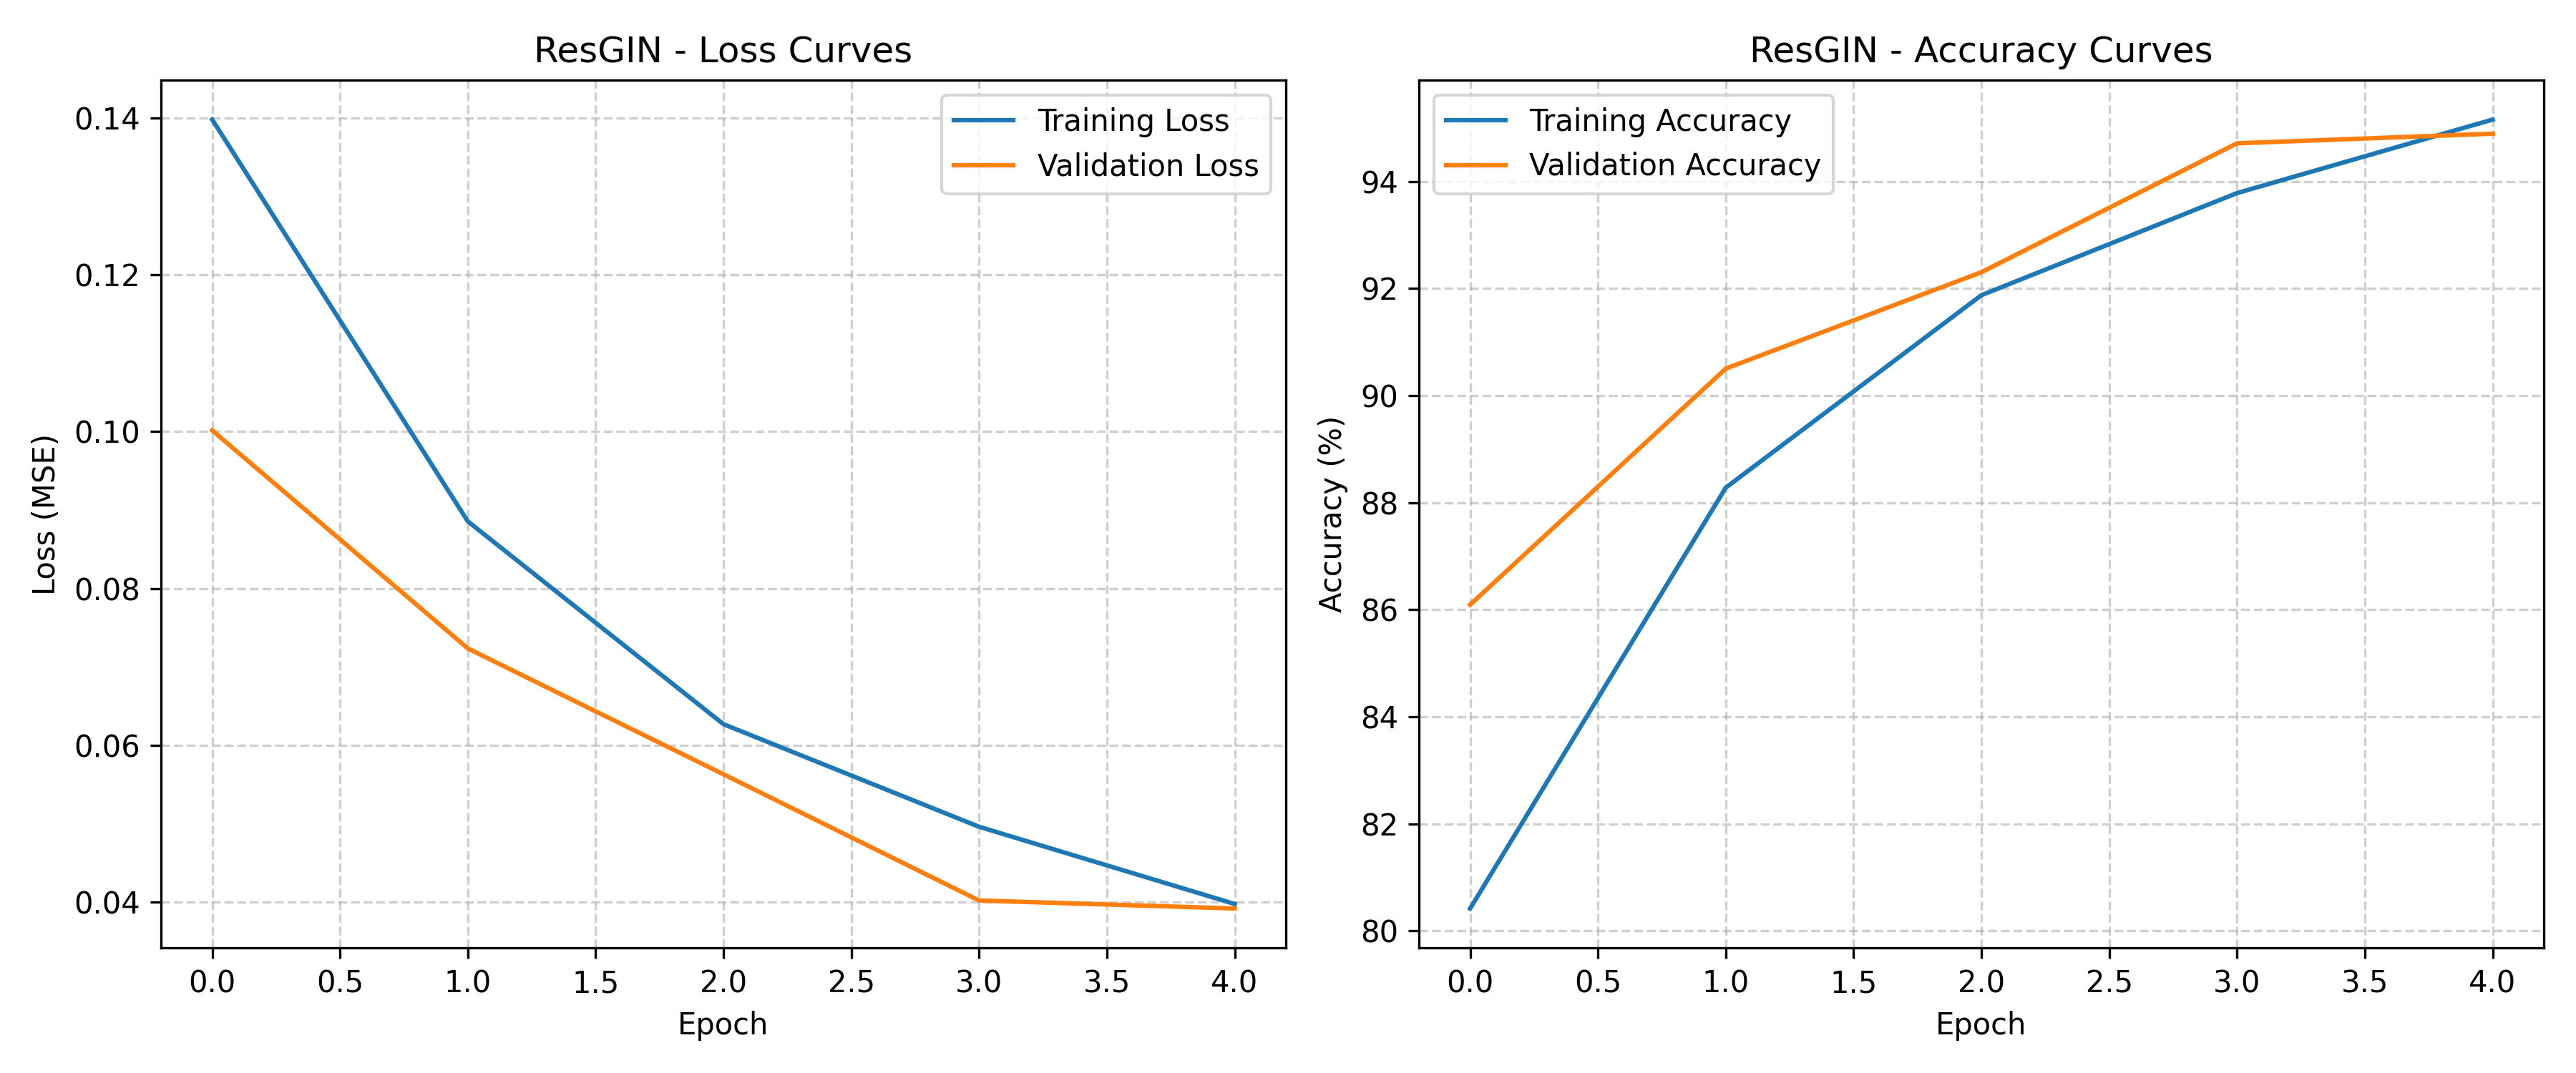
\includegraphics[width=0.8\linewidth]{resgin_test/ResGIN_learning_curves.png}
\caption{Learning curves of the ResGIN model during 5-epoch training, showing loss (left) and accuracy (right) for both training and validation sets.}
\label{fig:learning_curves}
\end{figure}

\subsection{ROC Curve Analysis}
Fig. \ref{fig:roc_curve} shows the Receiver Operating Characteristic (ROC) curve for the ResGIN model after 5 epochs of training. The high area under the curve (AUROC = 0.9768) indicates strong discriminative ability between interacting and non-interacting protein pairs.

\begin{figure}[htbp]
\centering
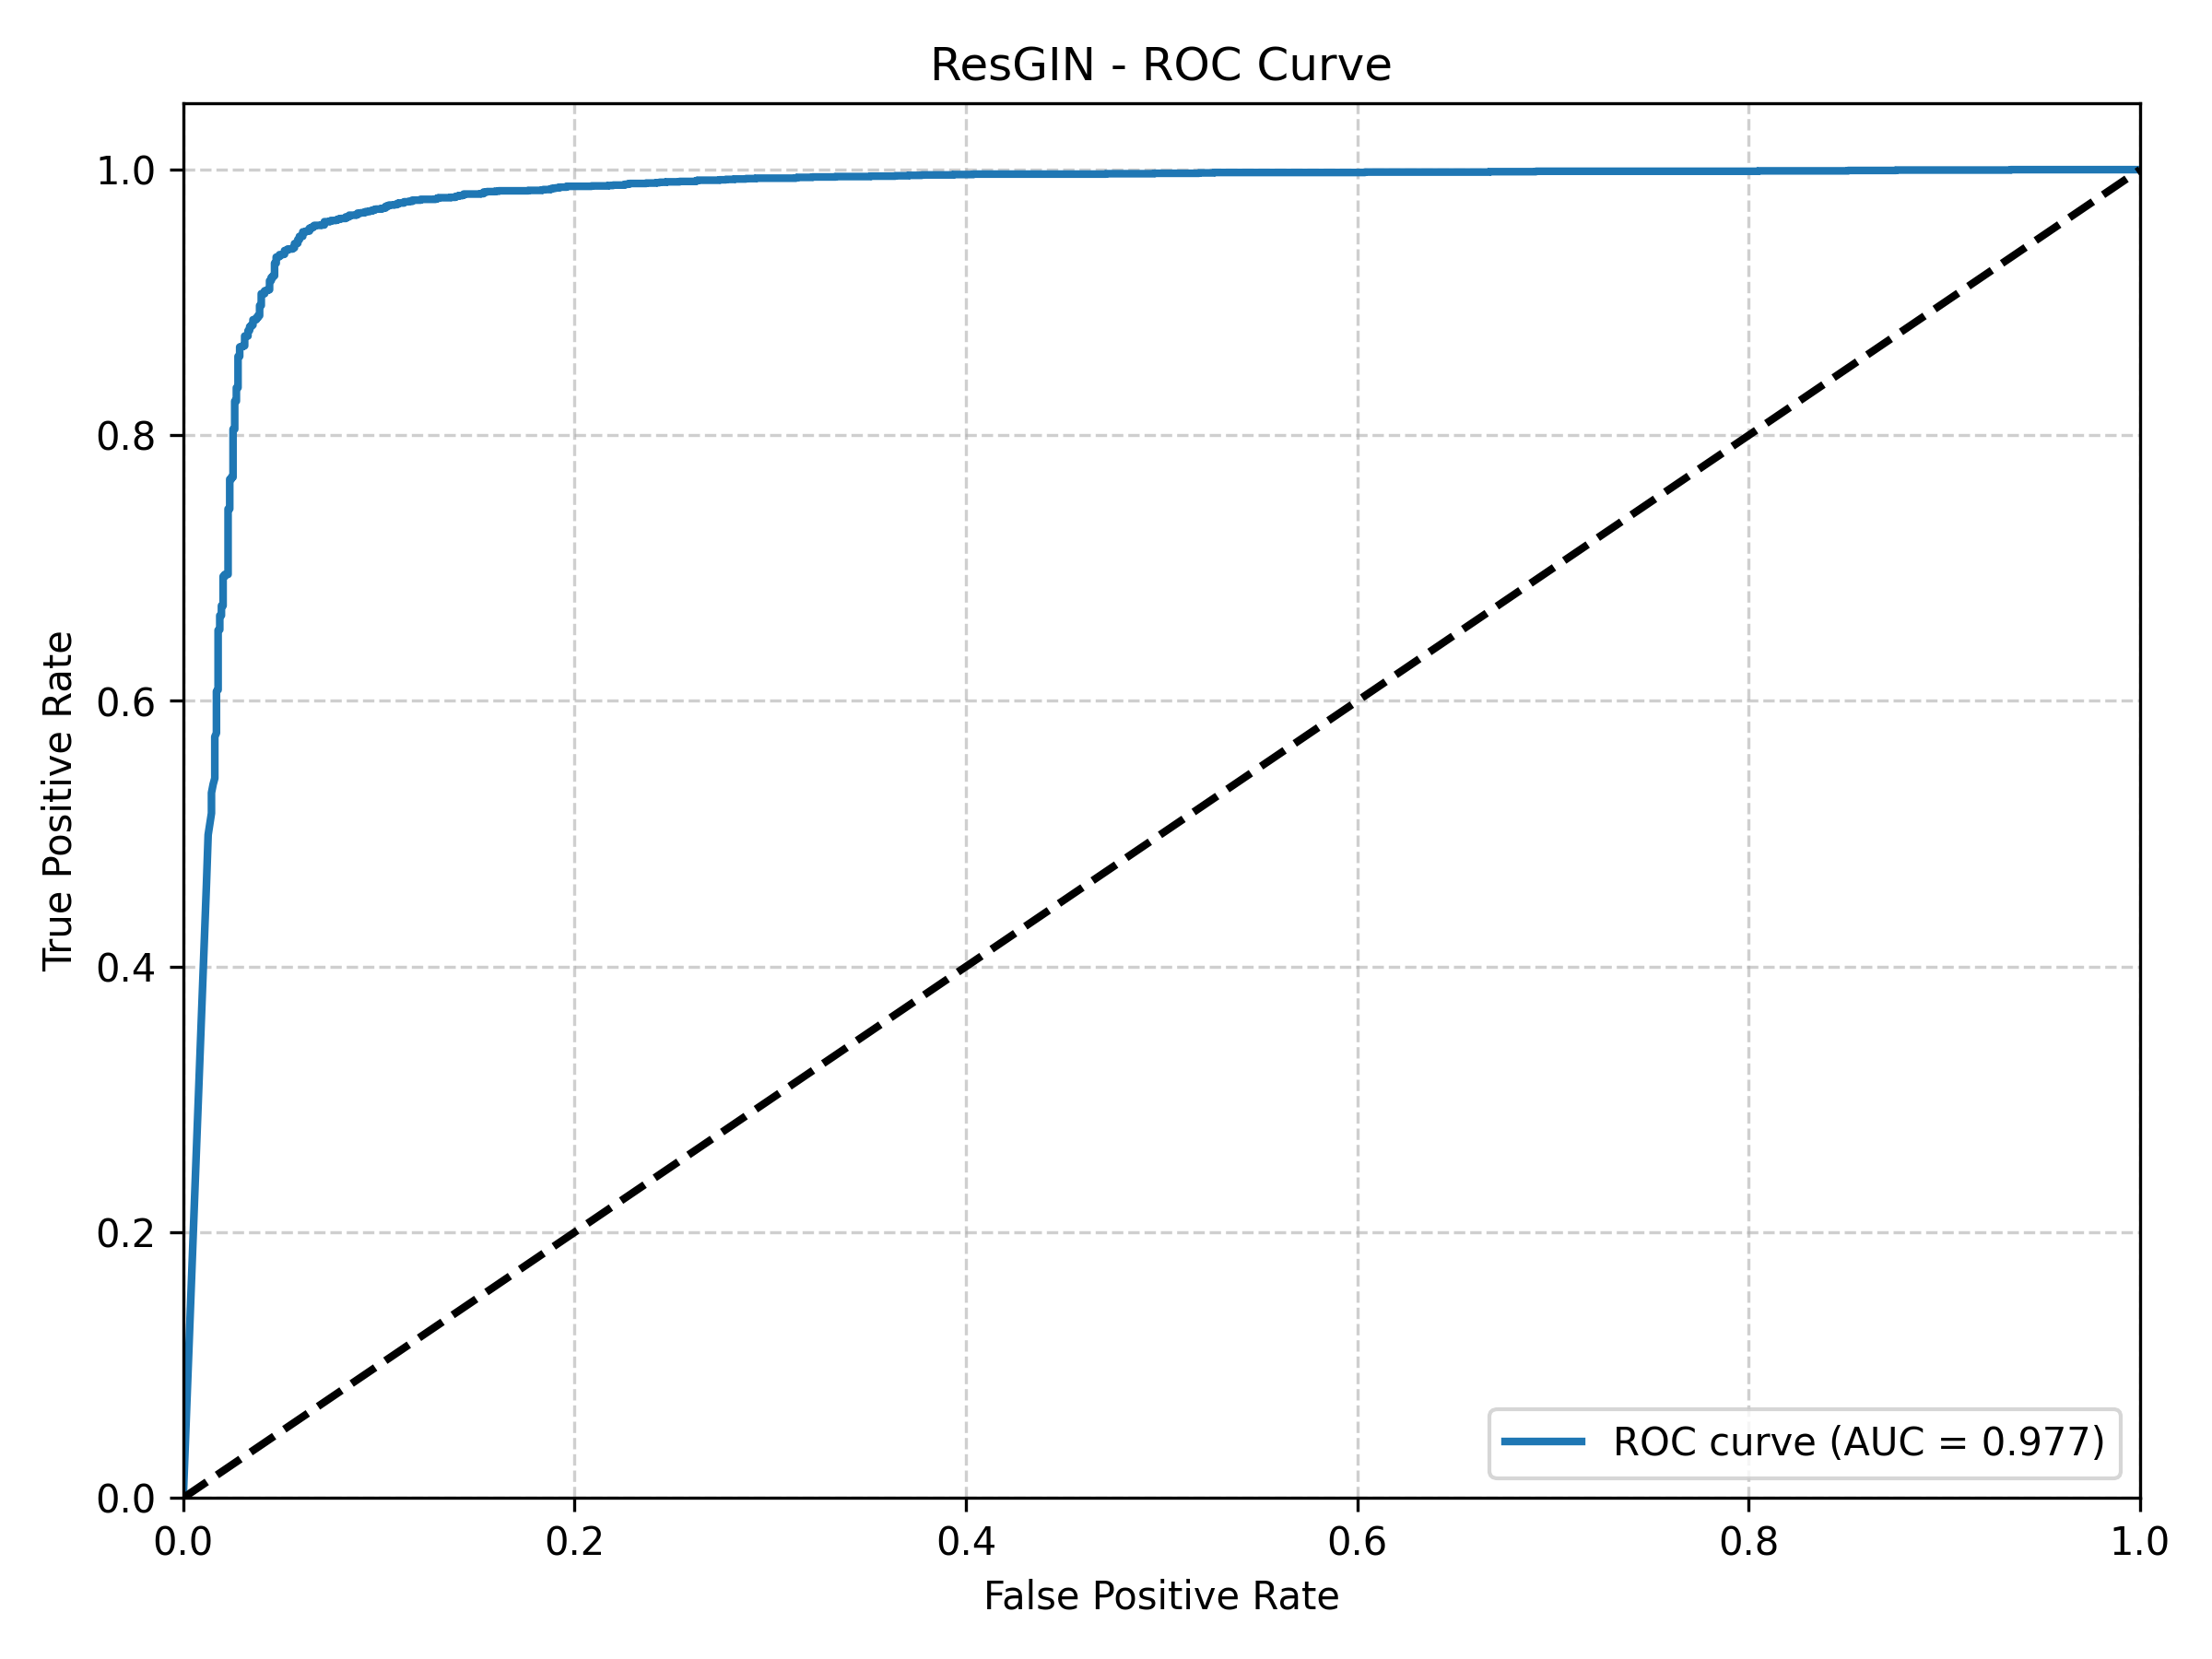
\includegraphics[width=0.5\linewidth]{resgin_test/ResGIN_roc_curve.png}
\caption{ROC curve for the ResGIN model, showing an AUROC of 0.9768.}
\label{fig:roc_curve}
\end{figure}

\subsection{Model Strengths and Limitations}

\subsubsection{ResGIN Strengths}
\begin{itemize}
    \item \textbf{Strong representational capacity}: The GIN layers provide powerful structural feature extraction capabilities.
    \item \textbf{Efficient learning}: Achieves high performance metrics with limited training.
    \item \textbf{Gradient flow}: Residual connections enable better gradient propagation, potentially benefiting deeper architectures.
    \item \textbf{Regularization}: Batch normalization layers contribute to stable training and help prevent overfitting.
\end{itemize}

\subsubsection{ResGIN Limitations}
\begin{itemize}
    \item \textbf{Computational complexity}: The multiple GIN layers with MLPs increase the computational cost compared to simpler GNN architectures.
    \item \textbf{Training time}: The model may require more training epochs to reach its full potential compared to GCNN.
\end{itemize}

\subsection{Architectural Insights}
The performance of ResGIN highlights the potential benefits of combining GIN's powerful expressiveness with residual connections. While GIN layers excel at distinguishing graph structures, they can become more challenging to optimize as networks deepen. The residual connections mitigate this issue by providing alternate pathways for gradient flow.

The GCNN model shows better short-term learning efficiency, achieving higher metrics after the same number of training epochs. This suggests that the simpler architecture may be more suitable for scenarios where training resources are limited, or when working with smaller datasets.

The AttGNN model demonstrates the best overall performance, but requires significantly more training epochs. The attention mechanism allows for dynamic weighting of neighboring nodes' features, which may capture more nuanced relationships in the protein structures.

\section{Conclusion and Future Work}
In this paper, we introduced ResGIN, a novel architecture that combines Graph Isomorphism Networks with residual connections for protein-protein interaction prediction. Our experimental results demonstrate that ResGIN achieves competitive performance compared to established GNN architectures, even with limited training epochs.

The performance of ResGIN suggests that the combination of GIN's discriminative power with residual connections creates a powerful model for capturing the complex structural patterns relevant to protein-protein interactions. With further optimization and extended training, ResGIN has the potential to match or exceed the performance of more established architectures.

Future work should explore several promising directions:

\begin{itemize}
    \item \textbf{Extended training}: Evaluate ResGIN's performance with longer training periods to assess its full potential
    \item \textbf{Hyperparameter optimization}: Conduct a systematic search for optimal hyperparameters, especially the number of GIN layers and their dimensions
    \item \textbf{Architectural variants}: Investigate hybrid architectures that combine ResGIN with attention mechanisms
    \item \textbf{Application to other datasets}: Test the model's generalization capability on different PPI datasets and across species
    \item \textbf{Explainability}: Develop methods to interpret the features learned by ResGIN to gain biological insights
\end{itemize}

Overall, our work contributes a promising new architectural approach to the field of PPI prediction using graph neural networks. The ResGIN model provides a strong foundation for future research in this important area of computational biology.

\bibliographystyle{IEEEtran}
\begin{thebibliography}{00}
\bibitem{skrabanek2008computational} Skrabanek, L., Saini, H. K., Bader, G. D., \& Enright, A. J. (2008). Computational prediction of protein–protein interactions. Molecular biotechnology, 38(1), 1-17.

\bibitem{gainza2020deciphering} Gainza, P., Sverrisson, F., Monti, F., Rodola, E., Boscaini, D., Bronstein, M. M., \& Correia, B. E. (2020). Deciphering interaction fingerprints from protein molecular surfaces using geometric deep learning. Nature Methods, 17(2), 184-192.

\bibitem{kipf2017semi} Kipf, T. N., \& Welling, M. (2017). Semi-supervised classification with graph convolutional networks. International Conference on Learning Representations (ICLR).

\bibitem{velivckovic2018graph} Veličković, P., Cucurull, G., Casanova, A., Romero, A., Lio, P., \& Bengio, Y. (2018). Graph attention networks. International Conference on Learning Representations (ICLR).

\bibitem{xu2018powerful} Xu, K., Hu, W., Leskovec, J., \& Jegelka, S. (2018). How powerful are graph neural networks? International Conference on Learning Representations (ICLR).

\bibitem{he2016deep} He, K., Zhang, X., Ren, S., \& Sun, J. (2016). Deep residual learning for image recognition. Proceedings of the IEEE Conference on Computer Vision and Pattern Recognition (CVPR), 770-778.

\bibitem{fout2017protein} Fout, A., Byrd, J., Shariat, B., \& Ben-Hur, A. (2017). Protein interface prediction using graph convolutional networks. Advances in Neural Information Processing Systems (NIPS), 6530-6539.

\bibitem{gligorijevic2019structure} Gligorijevic, V., Renfrew, P. D., Kosciolek, T., Leman, J. K., Berenberg, D., Vatanen, T., ... \& Bonneau, R. (2019). Structure-based protein function prediction using graph convolutional networks. bioRxiv, 786236.

\bibitem{li2019deepgcns} Li, G., Müller, M., Thabet, A., \& Ghanem, B. (2019). Deepgcns: Can gcns go as deep as cnns?. Proceedings of the IEEE International Conference on Computer Vision (ICCV), 9267-9276.

\bibitem{heinzinger2019modeling} Heinzinger, M., Elnaggar, A., Wang, Y., Dallago, C., Nechaev, D., Matthes, F., \& Rost, B. (2019). Modeling aspects of the language of life through transfer-learning protein sequences. BMC bioinformatics, 20(1), 1-17.

\bibitem{liu2019variance} Liu, L., Jiang, H., He, P., Chen, W., Liu, X., Gao, J., \& Han, J. (2019). On the variance of the adaptive learning rate and beyond. arXiv preprint arXiv:1908.03265.

\end{thebibliography}

\end{document}